\chapter{DSDV}
\label{chap:dsdv}

\section{Ejercicio 2.1}

\subsection{Avanza la simulación hasta el instante t = 7 s. Busca el primer paquete Hello transmitido a partir a ese
instante con un valor de hopdistance de al menos 3 y muestra una captura del contenido. Explica el significado
de los campos srcAddress y nextAddress, utilizando para explicarlos una captura de la tabla de enrutamiento del
nodo que está transmitiendo el paquete (i.e., no el que consta en srcAddress)}

\begin{figure}[H]
    \centering
    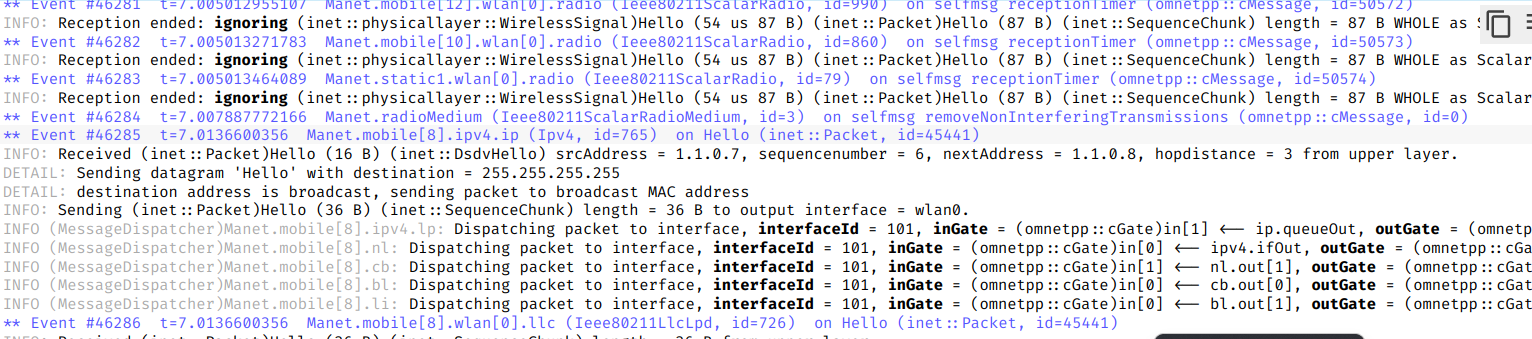
\includegraphics[width=155mm, scale=0.75]{imaxes/dsdv/ejercicio2_1.png}
    \caption{Log del nodo que manda el primer Hello con hopdistance 3}
    \label{fig:ejer2_1}
\end{figure}

Como se puede ver la imagen, el nodo que manda el primer mensaje Hello con hopdistance 1 es el nodo 8. Vamos a fijarnos en su tabla de enrutamiento:

\begin{figure}[H]
    \centering
    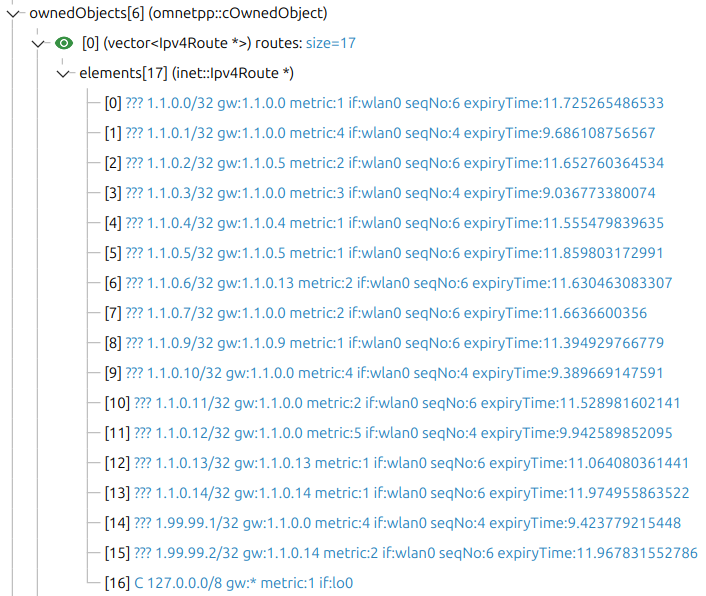
\includegraphics[width=115mm, scale=0.75]{imaxes/dsdv/ejercicio2_1_2.png}
    \caption{Tabla de enrutamiento nodo 8}
    \label{fig:ejer2_1_2}
\end{figure}

Según la imagen \ref{fig:ejer2_1}, el campo srcAddress es el nodo que generó el paquete Hello, en este caso es el 1.1.0.7 y el campo nextAddress es la siguiente dirección que va a retransmitir la trama, en este caso 1.1.0.8. 



\section{Ejercicio 2.2}

\subsection{¿Qué valor tiene de sequencenumber? ¿Qué quiere decir ese valor?}

Como se puede ver en la imagen \ref{fig:ejer2_1}, el campo sequencenumber tiene valor 6. Este valor ayuda a identificar entradas obsoletas para asi evitar bucles. Para ver si una ruta es válida o obsoleta llega con ver si este valor es par (ruta disponible) o impar (ruta obsoleta/caída). De esta forma, nos indica como de actualizado está la información de la ruta, el estado de la ruta y evita posibles conflictos en la red.

\section{Ejercicio 2.3}

\subsection{¿Cómo se modifica? ¿Qué nodo lo modifica, y cuándo lo hace?}

Este valor lo modifica el propio nodo en su tabla de enrutamiento, incrementándolo en 2 cuando la ruta que es válida o si es inválida solamente lo incrementa a 1. 
El nodo actualiza este valor cuando descubre una ruta mejor hacia el destino. Si el nuevo número de secuencia recibido es mayor (y par), el nodo adopta ese valor, lo registra en su tabla y actualiza el próximo salto (nextAddress) con el nodo que recibió la información (en este caso mobile[8]). En el caso de una ruta no válida, genera un sequencenumber impar y establece el costo de la ruta como infinito para indicar que esa ruta no se puede usar.  

\section{Ejercicio 2.4}

\subsection{Muestra la tabla de enrutamiento del nodo que recibe el Hello de la pregunta anterior justo antes y justo
después de recibirlo, relacionándola con el contenido del paquete. Si se actualiza la tabla, explica por qué se
actualiza y las entradas que se crean. Si no se actualiza, explica por qué no se actualiza y di qué entrada se
crearía (destino, gateway, métrica) si se actualizase con la información del paquete.}

\section{Ejercicio 2.5}

\subsection{Avanza hasta la caída del nodo en t = 15 s. Ten en cuenta que la ruta en ese momento puede ser diferente a
la de AODV, y por lo tanto el nodo a desactivar también. ¿Cuál es el primer nodo en darse cuenta de la caída?
¿Notifica la caída del nodo de alguna forma?}

Hay que aclarar que hemos cambiado de semilla ya que con DSDV no funcionaba bien con la semilla que usamos en los anteriores apartados.



\section{Ejercicio 2.6}

\subsection{¿Cómo se repara la ruta entre static1 y static2? ¿En qué momento?}



non recibe toda a tabla de enrutamiento cando si que deberia, algunhas veces os nodos mandan unha entrada da sua tabla, outras veces manda varias entradas...